\subsection{Succesive loop closure}


To simplify successive loop closure we can approximate the inner loops to gain = 1 for frequencies below the inner-loops bandwidth. 

\subsubsection{Roll loop}
For the inner most loop we will use equations (6.7) and (6.9) in the book.
\begin{equation*}
    k_{p_\phi} = \frac{\delta^{max}_a}{e^{max}_\phi} \text{sgn}(a_{\phi_2})
\end{equation*} and 
\begin{equation*}
    k_{d_\phi} = \frac{2 \zeta_\phi \omega_{n_\phi} - a_{\phi_1}}{a_{\phi_2}}
\end{equation*}

This gives us 
\begin{equation*}
    k_{p_\phi} = -\frac{5}{3}, k_{d_\phi} = -3.75
\end{equation*}

Now we want to find $k_{i_\phi}$ using root locus techniques. The transfer function with integral action $$H_{\phi/\phi_c} = \frac{k_{p_\phi}a_{\phi_2}s + k_{i_\phi}a_{\phi_2}}{s^3 + s^2(a_{\phi_1} + k_{d_\phi} a_{\phi_2}) + k_{p_\phi}a_{\phi_2}s + a_{\phi_2} k_{i_\phi}}$$ is derived in problem 2.4. 
The poles are 
\begin{equations}
    \begin{align*}
        0 &=s^3 + s^2(a_{\phi_1} + k_{d_\phi} a_{\phi_2}) + k_{p_\phi}a_{\phi_2}s + a_{\phi_2} k_{i_\phi} \\
        &= 1 + k_{i_\phi} \Big( \frac{a_{\phi_2}}{s(s^2 + (a_{\phi_1} + a_{\phi_2}k_{d_\phi})s + a_{\phi_2} k_{p_\phi})}  \Big)
    \end{align*}
\end{equations}
See listing \ref{lst:root_locus} for the MATLAB code. 
\todo[inline]{This is incorrect. Constants might be wrong.}

From figure \ref{fig:root_locus} we can derive a suitable interval for $k_{i_\phi}$.
\todo[inline]{Derive a suitable interval for this gain.}
\begin{figure}[h!]
    \centering
    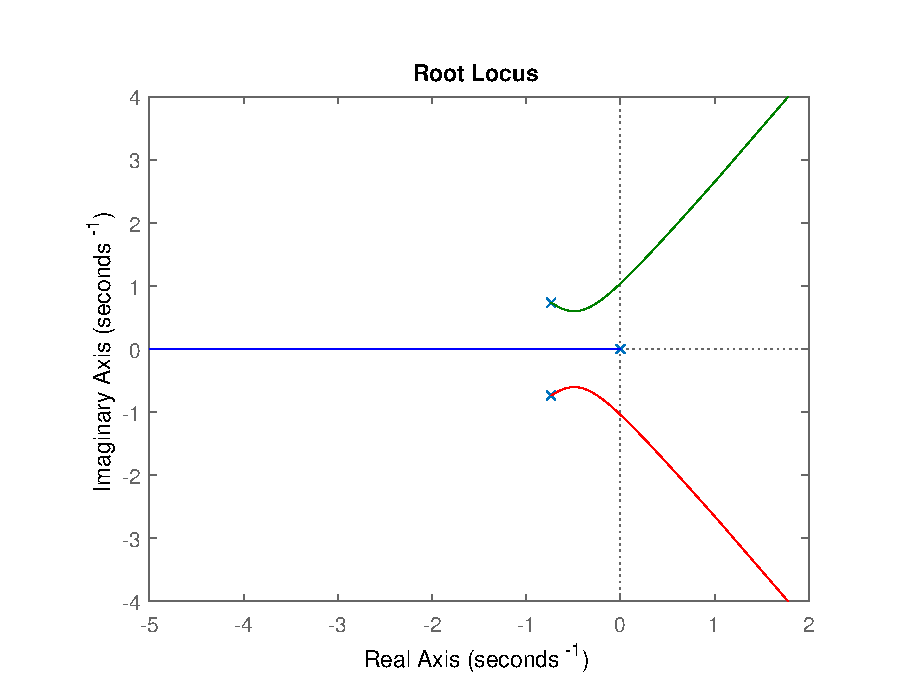
\includegraphics[scale=0.85]{rootLocus_kphi.eps}
    \caption{Root locus plot}
    \label{fig:root_locus}
\end{figure}

\subsubsection{Course loop}

Now let's look at the course loop. \\Here we have approximated the roll loop to one. See figure \ref{fig:course_loop} for the approximated block diagram.\\
We will use equations (6.12) and (6.13) in the book \cite{beard}.
\begin{equation*}
    k_{p_\chi} = \frac{2 \zeta_\chi \omega_{n_\chi} V_g}{g}
    \quad\text{and}\quad
    k_{i_\chi} = \frac{\omega^2_{n_\chi}V_g}{g}
\end{equation*}

To compute numerical values of the gains, we need numerical values of $\zeta_\chi$ and $\omega_n_\chi$. $\zeta_\chi$ is chosen to be 1 and $\omega_n_\chi$ is given by the following equation, where $W_x$ is chosen to be greater than 5. This is to assure sufficient bandwidth separation between the inner and outer loop:
\begin{equation*}
    \omega_n_\chi &= \frac{1}{W_\chi} \omega_n_\phi
    = \frac{1}{W_x} \sqrt{|a_\phi_2|\frac{\delta_a^{max}}{e_\phi^{max}}}
    = \frac{1}{6} \sqrt{0.65\frac{25}{15}}
    \approx 0.16 
\end{equation*}

We can now find the remaining gains:

\begin{equations}
    \begin{align*}
        k_{p_\chi} &= \frac{2 \zeta_\chi \omega_{n_\chi} V_g}{g} \approx 5.77\\
        k_{i_\chi} &= \frac{\omega^2_{n_\chi}V_g}{g} \approx 0.54
    \end{align*}
\end{equations}